\documentclass[12pt]{article}

\usepackage{times}
\usepackage{url}
\usepackage{graphicx}
\usepackage{amsmath}
\usepackage{tikz}
\usetikzlibrary{automata, arrows, positioning, calc}
\usepackage{color}

\setlength{\textwidth}{6.5in}
\setlength{\textheight}{8.9in}
\setlength{\oddsidemargin}{0.0in}
\setlength{\topmargin}{0.05in}
\setlength{\headheight}{-0.05in}
\setlength{\headsep}{0.0in}

\begin{document}

\begin{center}
{\bf CS 6300} \hfill {\large\bf HW4: Value Iteration} \hfill {\bf Due February 21, 2017}
\end{center}

\noindent
Please use the \LaTeX\ template to produce your writeups. See the
Homework Assignments page on the class website for details.  Hand in
at: \url{https://webhandin.eng.utah.edu/index.php}.

\section{Value Iteration}

At the AI casino, there are two things to do: Eat Buffet and Play AI
Blackjack.  You start out Poor and Hungry, and would like to leave the
casino Rich and Full.  If you Play while you are Full you are more
likely to become Rich, but if you are Poor you may have a hard time
becoming Full on your budget.  We can model your decision making
process as the following MDP:

\begin{flushleft}
\begin{tabular}{ll}
State Space & \{PoorHungry, PoorFull, RichHungry, RichFull\} \\
Actions     & \{Eat, Play\} \\
Initial State &  PoorHungry \\
Terminal State & RichFull 
\end{tabular}
\end{flushleft}

\begin{center}
\begin{tabular}{cc}
\begin{tabular}{|l|l|l|l|} \hline
$s$        & $a$  & $s'$       & $T(s,a,s')$ \\ \hline
PoorHungry & Play & PoorHungry & 0.8 \\ \hline
PoorHungry & Play & RichHungry & 0.2 \\ \hline
PoorHungry & Eat  & PoorHungry & 0.8 \\ \hline
PoorHungry & Eat  & PoorFull   & 0.2 \\ \hline
PoorFull   & Play & PoorFull   & 0.5 \\ \hline
PoorFull   & Play & RichFull   & 0.5 \\ \hline
RichHungry & Eat  & RichHungry & 0.2 \\ \hline
RichHungry & Eat  &RichFull    & 0.8 \\ \hline
\end{tabular} &
\begin{tabular}{|l|l|}\hline
$s'$       & $R(s')$ \\ \hline
PoorHungry & -1 \\  \hline
PoorFull   &  1 \\ \hline
RichHungry &  0 \\ \hline
RichFull   &  5 \\ \hline
\end{tabular} \\
Transition Model & Rewards
\end{tabular}
\end{center}

\begin{center}
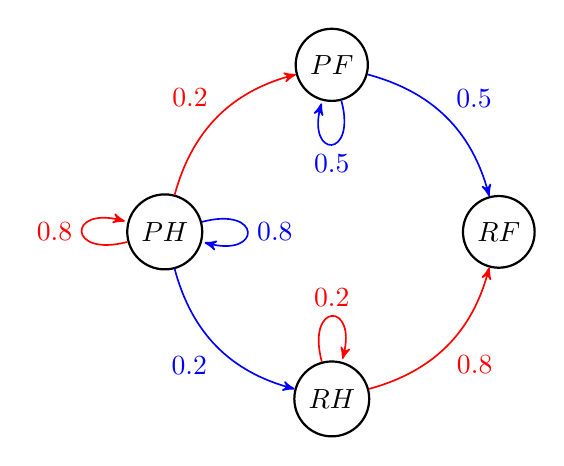
\begin{tikzpicture}[->, >=stealth', auto, semithick, node distance=3cm]
\tikzstyle{every state}=[fill=white,draw=black,thick,text=black,scale=1]
\node[state]    (PH)                     {$PH$};
\node[state]    (PF)[above right of=PH]   {$PF$};
\node[state]    (RH)[below right of=PH]   {$RH$};
\node[state]    (RF)[below right of=PF]   {$RF$};
\path
(PH) edge[loop left, red]     node{$0.8$}         (PH)
     edge[loop right, blue]   node{$0.8$}         (PH)
     edge[bend left, red]     node{$0.2$}         (PF)
     edge[bend right, blue]     node[below left]{$0.2$}       (RH)
(PF) edge[loop below, blue]    node{$0.5$}         (PF)
     edge[bend left, blue]    node{$0.5$}        (RF)
(RH) edge[loop above, red]    node{$0.2$}        (RH)
     edge[bend right, red]     node[below right]{$0.8$}        (RF);
\end{tikzpicture}

Where {\color{red}{red}} denotes the action to {\color{red}{Eat}} and {\color{blue}{blue}} denotes {\color{blue}{Play}}.
\end{center}

\newpage
\begin{enumerate}

\item Complete the table for the first 3 iterations of Value
  Iteration. Assume $\gamma = 1$.

\begin{center}
\begin{tabular}{|l|c|c|c|c|} \hline
State      & $i=0$ & $i=1$ & $i=2$ & $i=3$ \\ \hline \hline
PoorHungry &$\phantom{-}0.000$&$-0.600$&$-0.480$&$-0.084$\\ \hline
PoorFull   &$\phantom{-}0.000$&$\phantom{-}3.000$&$\phantom{-}4.500$&$\phantom{-}5.250$\\ \hline
RichHungry &$\phantom{-}0.000$&$\phantom{-}4.000$&$\phantom{-}4.800$&$\phantom{-}4.960$\\ \hline
RichFull   &$\phantom{-}0.000$&$\phantom{-}0.000$&$\phantom{-}0.000$&$\phantom{-}0.000$\\ \hline
\end{tabular}
\end{center}

The equation used is the {\em Bellman Update} Equation which is defined as

\[
   Q_{i+1}^{*}(s,a) = \sum_{s^{\prime}}T(s, a, s^{\prime})\left[ R(s, a, s^{\prime}) + \gamma\max_{a}Q^{*}_{i}(s^{\prime})\right]
\]

The values of {\em PoorHungry} ($PH$) is calculated for two iterations to show the steps.

\begin{align*}
Q_{1}(PH) &= 0.8(-1 + 0) + \max_{a}\left\{ \begin{array}{l} 0.2(1 + 0) = -0.60\\ 0.2(0 + 0) = -0.80\\\end{array}\right.\\
Q_{2}(PH) &= 0.8(-1 - 0.6) + \max_{a}\left\{ \begin{array}{l} 0.2(1 + 3) = -0.48\\ 0.2(0 + 4) = -0.48\\\end{array}\right.
\end{align*}

\item Assuming that we are acting for three time steps, what is the
  optimal action to take from the starting state? Justify your answer.

After 3 iterations, the Q-values have converged enough to where we can make a reasonable decision on the action that should be taken. From the above table, we can see that the best action to be chosen is to {\em Eat}, as the expected return value of {\em PoorFull} is $5.250$ compared to the value of $4.960$. 

This is expected as we can get ``more'' by taking $PF$, as there is a reward on reaching that state, even if looping back, compared to $R(RH) = 0$. 

As the number of iterations approaches infinity, the system converges such that $Q_{\infty}(PH) = 3.0$, $Q_{\infty}(PF) = 6.0$, and $Q_{\infty}(RH) = 5.0$. 
\end{enumerate}

\end{document}
